\documentclass[a4paper]{article}
\usepackage[spanish]{babel}
\usepackage[utf8]{inputenc}
\usepackage{fancyhdr}
\usepackage{charter}   % tipografia
\usepackage{graphicx}
\usepackage{makeidx}

\usepackage{float}
\usepackage{amsmath, amsthm, amssymb}
\usepackage{amsfonts}
\usepackage{sectsty}
\usepackage{wrapfig}
\usepackage{listings}
\usepackage{caption}

\usepackage{hyperref} %las entradas del índice tienen links
\hypersetup{
    colorlinks=true,
    linktoc=all,
    citecolor=black,
    filecolor=black,
    linkcolor=black,
    urlcolor=black
}

\usepackage{color} % para snipets de codigo coloreados
\usepackage{fancybox}  % para el sbox de los snipets de codigo

\definecolor{litegrey}{gray}{0.94}

% \newenvironment{sidebar}{%
% 	\begin{Sbox}\begin{minipage}{.85\textwidth}}%
% 	{\end{minipage}\end{Sbox}%
% 		\begin{center}\setlength{\fboxsep}{6pt}%
% 		\shadowbox{\TheSbox}\end{center}}
% \newenvironment{warning}{%
% 	\begin{Sbox}\begin{minipage}{.85\textwidth}\sffamily\lite\small\RaggedRight}%
% 	{\end{minipage}\end{Sbox}%
% 		\begin{center}\setlength{\fboxsep}{6pt}%
% 		\colorbox{litegrey}{\TheSbox}\end{center}}

\newenvironment{codesnippet}{%
	\begin{Sbox}\begin{minipage}{\textwidth}\sffamily\small}%
	{\end{minipage}\end{Sbox}%
		\begin{center}%
		\colorbox{litegrey}{\TheSbox}\end{center}}



\usepackage{fancyhdr}
\pagestyle{fancy}

%\renewcommand{\chaptermark}[1]{\markboth{#1}{}}
\renewcommand{\sectionmark}[1]{\markright{\thesection\ - #1}}

\fancyhf{}

\fancyhead[LO]{Sección \rightmark} % \thesection\
\fancyfoot[LO]{\small{Pablo González Alba, Nicolás Quiroz, Agustín Vaghi, Lucas Vuotto}}
\fancyfoot[RO]{\thepage}
\renewcommand{\headrulewidth}{0.5pt}
\renewcommand{\footrulewidth}{0.5pt}
\setlength{\hoffset}{-0.8in}
\setlength{\textwidth}{16cm}
%\setlength{\hoffset}{-1.1cm}
%\setlength{\textwidth}{16cm}
\setlength{\headsep}{0.5cm}
\setlength{\textheight}{25cm}
\setlength{\voffset}{-0.7in}
\setlength{\headwidth}{\textwidth}
\setlength{\headheight}{13.1pt}

\renewcommand{\baselinestretch}{1.1}  % line spacing


\usepackage{underscore}
\usepackage{caratula}
\usepackage{url}

\usepackage{color}
\usepackage{clrscode3e} % para el pseudocodigo




\begin{document}

\lstset{
  language=C++,
  backgroundcolor=\color{white},   % choose the background color
  basicstyle=\footnotesize,        % size of fonts used for the code
  breaklines=true,                 % automatic line breaking only at whitespace
  captionpos=b,                    % sets the caption-position to bottom
  commentstyle=\color{mygreen},    % comment style
  escapeinside={\%*}{*)},          % if you want to add LaTeX within your code
  keywordstyle=\color{blue},       % keyword style
  stringstyle=\color{mymauve},     % string literal style
}

\thispagestyle{empty}
\materia{Algoritmos y Estructuras de Datos III}
\submateria{Segundo Cuatrimestre de 2014}
\titulo{Trabajo Práctico I}
\subtitulo{Problemas de optimización}
\integrante{González Alba, Pablo}{476/10}{pablo.gonzalez.alba@gmail.com}
\integrante{Quiroz, Nicol\'as}{450/11}{nquiroz@dc.uba.ar}
\integrante{Vaghi, Agustín}{790/07}{vaghiagustin@gmail.com}
\integrante{Vuotto, Lucas}{385/12}{lvuotto@dc.uba.ar}

\maketitle
\newpage

\thispagestyle{empty}
\vfill
\begin{abstract}
    \vspace{0.5cm}
    En este trabajo práctico, resolveremos problemas de \textbf{optimización}, aplicando diferentes técnicas
    algorítmicas (como \textit{backtracking}, \textit{algoritmos golosos}, \textit{podas} en árboles, etc).
    Luego, realizaremos diferentes \textbf{análisis teóricos sobre la complejidad y correctitud} de los mismos. \medskip

    Finalmente pondremos nuestros algoritmos a prueba en \textbf{diferentes escenarios}, ilustrando con gráficos
    representativos y sacando conclusiones en base a los resultados obtenidos.
\end{abstract}

\thispagestyle{empty}
\vspace{1.5cm}
\tableofcontents
\newpage


%\normalsize
\newpage

\section{Objetivos generales}
\begin{itemize}
  \item Utilizar \textbf{diferentes técnicas algorítmicas} para resolver los problemas.

  \item Hallar una \textbf{solución óptima} para el problema. Esto implica que la complejidad de los
  algoritmos utilizados no supere cierta cota superior (salvo en el problema 3), en sus peores casos.

  \item Escribir el \textbf{pseudocódigo correspondiente a la solución} de cada problema y el código
  (basado en el anterior), utilizando las diferentes estructuras y \textit{contenedores} que nos
  brinda la \textit{STL} de C++, para simplificar el desarrollo.

  \item Justificar que las implementaciones utilizadas \textbf{resuelven efectivamente los problemas} y
  además son \textbf{correctas}.

  \item Realizar un \textbf{análisis de complejidad de los algoritmos propuestos}, mostrando que cumplen
  con las cotas pedidas.

  \item Realizar diferentes \textbf{experimentaciones y gráficos} que muestren el comportamiento de nuestros
  algoritmos para instancias variadas, contrastando esta información empírica con las demostraciones
  teóricas.
\end{itemize}

\newpage

\section{Plataforma de pruebas}
El testeo de los algoritmos implementados fue realizado, principalmente, en las máquinas del laboratorio 3 del DC. \newline
\begin{itemize}
  \item \textbf{Sistema Operativo:} Ubuntu Linux 12.04 x86_64, kernel 3.2.0-30-generic

  \item \textbf{Especificaciones del Software:} el código está implementado en \textbf{C++}, compilado con \verb|-std=c++0x|.
  Utilizamos \textbf{Bash} y \textbf{Ruby} para los scripts. Los gráficos fueron realizados con \textbf{gnuplot}.

  \item \textbf{Especificaciones del Hardware:} Intel(R) Core(TM) i5-2500K CPU @ 3.30GHz, 8GB de RAM.
\end{itemize}

\newpage

\section{Problema 1: Puentes sobre lava caliente}
\subsection{Descripción del problema.}

\vspace*{0.3cm}

Este problema se trata de implementar un algoritmo que, de ser posible,
\textbf{calcule la cantidad mínima de saltos} que debe dar un participante para poder cruzar un
puente de cierto tamaño (fijo), el cual presenta \textbf{algunos de sus tablones rotos}. Estos se encuentran
marcados y \textbf{deben ser evitados}, de otro modo, el participante fracasa en su intento y puede llegar a
perder la vida. Cada uno de los participantes puede saltar una \textbf{determinada cantidad de tablones como máximo}. \medskip

El algoritmo debe decidir si dicha hazaña es posible, y de ser así,
\textbf{especificar la cantidad de saltos a dar y a qué tablones hacerlo}. \medskip

Asumimos que tanto la \textbf{longitud del puente como la cantidad de saltos máximos por participante
son valores naturales}.

\vspace*{0.5cm}

\textbf{Ejemplos:}
\begin{itemize}
  \item Para un puente de 10 tablones y un participante capaz de saltar de a 3
  tablones como máximo, teniendo los tablones 1, 4, 6, 8 y 9 rotos, la salida podría ser:
  primero saltar al tablón 3, luego al 5, luego al 7, luego al 10 y luego fuera del puente.
  \item Si en cambio, en el ejemplo anterior, el tablón 7 también estuviese roto,
  el algoritmo debe informarnos que, bajo esas condiciones, no es posible cruzar el puente.
  \item \textcolor{red}{\textbf{agregar un ejemplo mas con dibujitos y cosas lindas!}}
\end{itemize}



\subsection{Desarrollo de la idea y pseudocódigo.}

\vspace*{0.3cm}

Para resolver este problema, propusimos un algoritmo de tipo \textit{greedy}, que en cada iteración
del mismo busca siempre saltar \textbf{la mayor cantidad posible de tablones}, siempre y cuando el
tablón al que nos dirijamos esté sano. Caso contrario, se saltará al tablón anterior (ó al anterior), 
y así sucesivamente, hasta encontrar un tablón válido.
Si retrocediendo de este modo se llega a la posición en la que se encuentran el competidor, el problema
\textbf{no tiene solución}.

\vspace*{0.5cm}


\begin{codebox}
\Procname{$\proc{cruzarPuente}(n,c,puente)$}
\li \Comment n: cantidad de tablones del puente puente es el vector
\li \Comment c: cantidad de tablones máximos a saltar
\li \Comment puente: es el conjunto de tablones
\li \Comment el primer tablón es el 1
\li $\id{solucion} \gets \emptyset$
\li \If $\id{c} > \id{n}$
\li     \Then
            $\proc{agregar}(solucion, c)$
\li         \Return $\id{solucion}$
        \End
\li \If $\neg(\proc{esPosibleCruzar}(puente, c))$
\li     \Then
            \Return $\emptyset$
        \End
\li $\id{posicionActual} \gets 0$
\li \While $\id{posicionActual} \leq \id{n}$
\li     \Do
            $saltoActual \gets c$
\li         \While $\neg(\proc{puedeSaltar}(puente, posicionActual + saltoActual - 1))$
\li         \Do
                $saltoActual \gets saltoActual - 1$
            \End
\li     $\id{posicionActual} \gets \id{posicionActual} + \id{saltoActual}$
\li     $\proc{agregar}(solucion, posicionActual)$
        \End
\li \Return $\id{solucion}$
\end{codebox}


\vspace*{0.5cm}


\begin{codebox}
\Procname{$\proc{puedeSaltar}(puente, tablon)$}
    \Return $\id{tablon} \geq \proc{tamanio}(puente) \lor \proc{estaSano}(puente[tablon])$
\end{codebox}


\vspace*{0.5cm}


\begin{codebox}
\Procname{$\proc{esPosibleCruzar}(puente, c)$}
\li \Comment c: cantidad de tablones máximos a saltar
\li $\id{tablonesRotosConsecutivos} \gets 0$
\li \For $i \gets 0$ \To $\proc{tamanio}(puente) - 1$
\li     \Do
            \If $\proc{puedeSaltar}(puente, i)$
\li             \Then
                    $\id{tablonesRotosConsecutivos} \gets 0$
\li         \Else
\li             $\id{tablonesRotosConsecutivos} \gets \id{tablonesRotosConsecutivos} + 1$
            \End
\li         \If $\id{tablonesRotosConsecutivos} \geq c$
\li             \Then
                    \Return $\const{false}$
            \End
        \End
\li \Return $\const{true}$
\end{codebox}



\subsection{Justificación de la resolución y demostración de correctitud.}

\vspace*{0.3cm}

Antes de comenzar, diremos que una solución $S$ es de la forma $s \ t_1 \dots t_s$,
siendo $s$ la cantidad de saltos y $t_i$ el $i$-ésimo tablón al cual saltar. $S$ se considera
\textit{óptima} si $s$ es \textbf{mínimo}. También definiremos la relación entre soluciones $\sqsubseteq$, que,
dadas $S = s \ t_1 \dots t_s$ y $H = h \ u_1 \dots u_h$, se da del siguiente modo:
\begin{align*}
  S \sqsubseteq H \iff s \leq h \wedge \bigwedge_{i=1}^s t_i = u_i
\end{align*}

Para demostrar que el algoritmo propuesto es correcto para la resolución de este problema,
separaremos las entradas en casos y analizaremos éstos a continuación.

\begin{itemize}
  \item $c > n$: en este caso, la solución será de la forma $1 \ k$, con $k > n$. Como $c > n$, la
  solución $1 \ c$ es una solución posible (y óptima).

  \item $c \leq n$: si la instancia no tiene solución, es porque hay $c$ o más tablones
  consecutivos rotos. En tal caso, la función \textsc{esPosibleCruzar} se encarga de
  decirnos si hay solución. Más adelante demostraremos que \textsc{esPosibleCruzar}
  también es correcta. \medskip

  En cambio, si tiene solución, plantearemos el siguiente esquema:

  \begin{codebox}
  \Procname{$\proc{Greedy}(S,f,p)$}
  \li \Comment $S$ es el conjunto de tablones
  \li \Comment $f$ es una función que elige el tablón mas lejano que se puede saltar
  \li \Comment $p(A, x)$ es una función que indica si a una subsolución $A$ se le
  \li \Comment   puede agregar el tablón $x$. Es decir, si está sano y a una distancia
  \li \Comment   a lo sumo igual al salto máximo del último tablón agregado.
  \li $\id{S^{opt}} \gets \emptyset$
  \li \While $\id{S} \neq \emptyset$
  \li     \Do
    			$\id{x} \gets f(S)$
  \li  			$\id{S} \gets \id{S} \setminus \{\id{x}\}$
  \li			\If $p(S^{opt}, x)$
    				\Then
  \li					$\id{S} \gets \id{S} \setminus \{\id{c} \mid \id{c} < \id{x}\}$
  \li					$\id{S^{opt}} \gets \id{S^{opt}} \cup \{\id{x}\}$
    				\End
    		\End
  \li \Return $\id{S^{opt}}$
  \end{codebox}

  \textbf{Demostración (\textsc{cruzarPuente}):}
  \begin{itemize}
    \item Definimos como \textbf{subsolución} a un conjunto de tablones, que
    es \textbf{subconjunto de una solución óptima}.
    \item $S^{opt}$ empieza siendo $\emptyset$, que es subconjunto de cualquier
    solución óptima (si tal solución existe). Inicialmente se calcula si
    existe forma de cruzar el puente, por lo que al llegar a este punto del
    algoritmo, se puede estar seguro que existe una solución.
    \item Supongamos que estamos en la iteración k-ésima. Al iniciar
    el ciclo, $S^{opt}$ es una subsolución de la solución óptima $S^{*}$. \medskip
    
    Sea $S^{opt} \sqsubseteq S^{*}$ y $\id{x} \gets F(S)$. \medskip
    
    En esta iteración, podemos: \medskip
    
    $(a)$ No agregar $x$ a $S^{opt}$
    
    $(b)$ Agregar $x$ a $S^{opt}$ \medskip
    
    Si sucede $(a)$, entonces no se modifica $S^{opt}$, por lo tanto sigue
    siendo \textbf{subsolución de $S^{*}$}, es decir, es una \textbf{solución óptima}. \medskip
    
    Si sucede $(b)$, agregamos $x$ (aplicamos $f(S)$), es decir, el tablón más
    lejano al cuál se puede saltar. Como lo estamos agregando, vale
    $p(S^{opt}, x)$, es decir, que $x$ es un tablón sano. \medskip
    
    Sea $S'^{opt} \gets S^{opt} \cup \{x\}$. Queremos ver que existe una
    solución óptima $S'^{*}$, tal que $S'^{opt} \sqsubseteq S'^{*}$. \medskip
    
    Tenemos, nuevamente, dos casos: \medskip 
    
    $(a')$ $x \in S^{*}$
    
    $(b')$ $x \notin S^{*}$ \medskip
    
    Si sucede $(a')$, entonces $S'^{opt} \sqsubseteq S^{*}$. 
    Tomamos $S'^{*} \gets S^{*}$, una solución óptima. \medskip 
    
    Caso $(b')$. Sean $x'$ el \textbf{mínimo valor} de $S^{*} \setminus S^{opt}$, 
    $u$ el máximo valor de $S^{opt}$ (es decir, la última posición a la que
    se saltó) y $u'$ el mínimo valor de $S^{*} \setminus (S^{opt} \setminus \{x'\})$, es
    decir, el valor siguiente a $x'$ en $S^{*}$.
    
    Como $x \notin S^{*}$, $x$ no puede ser igual a $x'$. Entonces $x' > x$.
    Pero el salto de $u$ hacia $x'$ es válido, porque $S^{*}$ es una solución
    válida. Es \textbf{absurdo}, porque definimos $f$ como la función que nos
    da la mayor posición válida y en este caso retornó $x$ en lugar de $x'$.
    
    Por lo tanto, sólo puede valer $x > x'$. En este caso, consideremos a
    $S'^{*} \gets S^{*} \setminus (\{x'\} \cup \{x\})$. El salto de $u$ hacia $x$ es
    válido, porque así lo indica $p(S^{opt}, x)$ y el salto de $x$ hacia $u'$
    es menor que el de $x'$ hacia $u'$. Por lo tanto, si el salto de $x'$ es válido,
    el de $x$ también. La cantidad de saltos de $S'^{*}$ es exactamente igual a la de 
    $S^{*}$, ya que consiste simplemente en reemplazar un elemento por otro.
    
    Entonces $S^{opt} \sqsubseteq S'^{*}$, es una \textbf{subsolución de una solución óptima}.
    
    \item Al terminar el ciclo, recorremos todos los tablones y vemos que $S^{opt}$ 
    es subsolución de una solución óptima. Sea $S^{*}$ tal solución óptima.
    Si $S \gets S^{*}$ entonces $S^{opt}$ es una solución óptima.
    
    Si no, $\exists x \in (S^{*} \setminus S^{opt})$. Pero $x \in S$ y $p(S^{*}, x) \gets \const{true}$,
    por lo tanto $p(S^{opt}, x) \gets \const{true}$ y $P(X, x) \gets \const{true}$, para todo prefijo
    X de $S^{opt}$. Entonces, al momento de sacar $x$ de $S$ e intentar agregarlo a $S^{opt}$, 
    deberíamos poder, pero no es lo que sucede. 
    
    Esto no puede pasar, luego no existe $x$, y $S^{*} \gets S^{opt}$.

  \end{itemize}

\newpage

\textbf{Demostración (\textsc{esPosibleCruzar}):} 
\begin{itemize}
\item La función \textsc{esPosibleCruzar} mantiene un \textbf{contador de tablones rotos consecutivos},
inicializado en 0. Recorre todos los tablones \textbf{en orden}; si el tablón actual
está sano, resetea el contador a 0, sino (está roto) le suma 1.
Luego, si en algún momento el contador es \textbf{mayor ó igual al salto máximo posible},
devuelve \textbf{falso}. En cambio, si se recorren todos los tablones y esto no sucede, 
la función devuelve \textbf{verdadero}.

Por lo tanto, la función devuelve falso $\iff$ existe en algún momento una
cantidad de tablones rotos consecutivos mayor o igual al salto máximo. 

Veamos que esto es equivalente a que el puente pueda ser cruzado: \medskip

\textbf{Teorema:} Es posible cruzar un puente $\iff$ su cantidad de tablones rotos
consecutivos es menor al salto máximo. \medskip

\item \textbf{Demostremos la ida:}
Sea un puente de $n$ tablones, con un salto máximo de $c$ y una cantidad máxima de
tablones rotos consecutivos $k$.
Supongamos $k \geq c$.
Si es posible cruzarlo, entonces existe una solución $S$, que consiste en una
secuencia de saltos.
Sean $t_1$ el primero de los tablones y $t_c$ el tablón correspondiente a la posición $c$, entre 
los tablones consecutivos rotos (que sabemos que existe porque c $\leq$ k).
Sea $s_0 \in S$ la posición (en tierra o en un tablón) máxima anterior a $t_1$ y sea $s_1 \in S$ 
la posición inmediata siguiente a $s_0$.
Dado que $c$ es el salto máximo, entonces $s_1 - s_0 \leq c$ ó, lo que es lo
mismo, $s_0 + c \geq s_1$.
Elegimos $s_0 < t_0$, entonces $s_0 + c < t_0 + c$.
Pero esto es $s_0 + c < t_c$ y $s_1 \leq s_0 + c < t_c$.

Entonces, o bien $s_1 < t_0$ (que resulta imposible, pues se eligió $s_0$ como el máximo
menor a $t_0$), ó $t_0 \leq s_1 < t_c$, pero entonces el salto se hubiera realizado a un
tablón roto. \medskip

\textbf{¡Absurdo!}, que viene de suponer que existe una solución cuando la cantidad de
tablones rotos consecutivos es igual o mayor al salto máximo. \medskip

\item \textbf{Demostremos la vuelta:}
Sea un puente de $n$ tablones, con salto máximo $c$ y cantidad máxima de
tablones rotos consecutivos $k$, con $k < c$.
Sea $S$ la solución que consiste en caer en todos los tablones sanos y luego al
otro lado del puente (es decir, cruzarlo).

Esta solución cruza el puente completamente y para cada posición 
$s_i \in S, 1 \leq s_{i+1} - s_i \leq k$, ya que no saltea tablones sanos.
Entonces $s_{i+1} - s_i \leq k => s_{i+1} - s_i \leq c$. 

Por lo tanto todos los saltos en $S$ son válidos y la solución existe.
\end{itemize}

\end{itemize}



\subsection{Análisis de complejidad.}

\vspace*{0.3cm}

Para el análisis de complejidad nos basaremos en el pseudocódigo de la función 
\textsc{cruzarPuente}, correspondiente al ítem \textbf{3.2}.

\begin{enumerate}
  \item Todas las operaciones realizadas sobre el contenedor \verb|vector| de la \textit{STL} (size, push_back, empty y la creación de iteradores)
  toman tiempo constante $O(1)$.

  \item Las asignaciones realizadas (11, 13, 15, 16 y 17) también se realizan en tiempo constante $O(1)$.

  \item Si $c$ es mayor que $n$ (línea 6), retornamos el vector de soluciones que contiene la cantidad de saltos realizados (cero) y
  el "tablón" $c$ hacia el cual saltamos. Como dijimos anteriormente, realizar estas operaciones sobre \verb|vector|
  toma tiempo constante $O(1)$.

  \item En la línea 9, ejecutamos el condicional \verb|esPosibleCruzar(puente, c)|. La complejidad de esta función la
  analizaremos luego, pero adelantamos que es lineal, $O(n)$.

  \item En la línea 12 (tener en cuenta que en este caso vale $c \leq n$), en el peor caso ($c = 1$), realizamos $n$ iteraciones,
  pues recorremos el puente de a un tablón (siempre y cuando no haya tablones rotos, pues no tendría solución). Con $c \neq n$,
  en cualquier iteración podemos realizar a lo sumo $c$ retrocesos, pero en las siguientes esto es compensado, pues sabiendo que
  hay solución, la metodología empleada no pregunta más de 1 vez el estado de un mismo tablón. Este procedimiento tiene como peores
  casos los siguientes:
  \begin{itemize}
    \item $c = 1$, con todos los tablones sanos, de manera que haya que chequear todos los tablones del puente.

    \item $c = 2$, con un patrón de tablones sano - roto - sano, como se puede ver en la figura \textcolor{red}{\textbf{QUE DESPUES AGREGAMOS!}}

    \item $c = n$, con todos los tablones rotos salvo el primero, de manera que haya que chequear todos los tablones del puente.
  \end{itemize}

  \item La complejidad de \verb|esPosibleCruzar(puente, c)| (línea 9) es $O(n)$, pues en el peor caso recorre el puente entero.

  \item La complejidad de \verb|puedeSaltar(puente, tablón)| es $O(1)$, pues obtenemos el tamaño del puente en tiempo constante
  mediante la función \verb|size| y preguntar si un tablón está sano ó no es constante.

\end{enumerate}

Por lo tanto, la \textbf{complejidad total} del algoritmo implementado para este problema es

\begin{align*}
  O(1) + O(1) + O(n) + O(n)*O(1) = \textit{\textbf{O(n)}}
\end{align*}



\subsection{Partes relevantes del código (hacer referencia al apéndice).}

\vspace*{0.3cm}

desarrollo.



\subsection{Experimentación y gráficos.}

\vspace*{0.3cm}

\subsubsection{Test 1 - distribución aleatoria de tablones}

En este test, fijamos el valor de $c$ (salto máximo) en 20, mientras que $n$ (cantidad de tablones) 
se inicializa en 1000 y va incrementándose también de a 1000, hasta alcanzar 1000000. La 
distribución de los tablones rotos/sanos se genera aleatoriamente, de forma uniforme. 
Se toma el valor mínimo de cantidad de ciclos luego de 25 corridas. 


\vspace*{0.5cm}


\subsubsection{Test 2 - }



\newpage

\section{Problema 2: Horizontes lejanos}
\subsection{Descripción del problema.}

\vspace*{0.3cm}

Dado un \textbf{tablero de ajedrez de tamaño $n$x$n$ y $k$ caballos ocupando
inicialmente ciertos casilleros (aleatorios)} del mismo, el objetivo consiste
en \textbf{reunir a todos los caballos en un mismo casillero, minimizando la
cantidad total de movimientos realizados}. Esta cantidad equivale a
\textbf{la suma de los movimientos de todos los caballos} en el tablero.

Un caballo $k$ puede moverse únicamente \textbf{respetando los movimientos
válidos según las reglas del ajedrez}. Además, \textbf{un casillero puede
estar ocupado por más de un caballo simultáneamente}.

\vspace*{0.5cm}

\textbf{Ejemplo:}

En un tablero de 8x8, con 3 caballos en las posiciones [2,2], [5,5] y [2,8],
la menor cantidad de saltos posibles es 4, haciendo que los caballos de los
extremos cayan hacia la posición del caballo del medio[5,5], como se puede ver
en la siguiente imagen:

\begin{figure}[htb]
  \begin{center}
      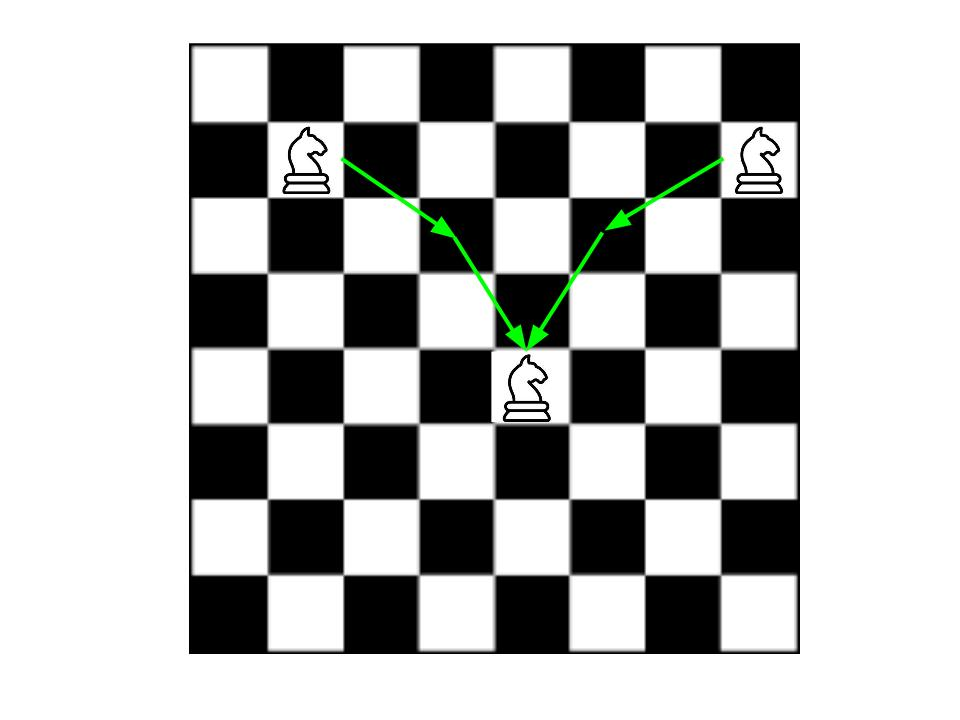
\includegraphics[scale=0.25]{imagenes/caballos.jpg}
  \end{center}
  \caption{ejemplo de tablero.}
\end{figure}


\newpage
\subsection{Desarrollo de la idea y pseudocódigo.}

\vspace*{0.3cm}


Para resolver este problema, utilizaremos $k$ tableros de $n$x$n$ casilleros,
uno por cada caballo. En cada tablero se calculará el costo para dicho caballo
de llegar a cada casillero, aplicando \textit{BFS} desde el casillero inicial,
quedando inválidos los casilleros que no pueden alcanzarse.

Luego se recorren todos los casilleros, sumando el valor de éstos en todos los
tableros (si son alcanzables), obteniendo así el costo de cada casillero para
cada caballo. De existir, el mínimo de estos valores será el casillero que
pueden alcanzar todos los caballos en la menor cantidad de saltos.

%\begin{codebox}
%\Procname{$\proc{puntoDeEncuentro}(caballos, n)$}
%\li $\id{tableros} \gets \emptyset$
%\li \For $caballo \in caballos$
%\li   \Do
%\li       $\proc{agregar}(\proc{crearTablero}(caballo,n), tableros)$
%      \End
%\li $\id{i} \gets 0$
%\li $\id{j} \gets 0$
%    $\id{min_i} \gets -1$
%    $\id{min_j} \gets -1$
%    $\id{min} \gets -1$
% \li \While $\id{i} < \id{n}$
% \li   \Do
% \li     \While $\id{j} < \id{n}$
% \li       \Do
% \li         $\id{sum} \gets 0$
% \li         $\id{caballo} \gets 0$
% \li         \While $\id{caballo} < \proc{tamaño}(caballos)$
% \li           \Do
%                 if (tableros[caballo][i][j] == -1)
%                   sum = -1
%                 else if (sum != -1)
%                   sum += tableros[caballo][i][j]
%                 end
%                 caballo++
%               \End
%             if (sum != -1 && (min == -1 || sum < min))
%               min = sum
%               min_i = i
%               min_j = j
%             end
%             j++
%         \End
%         i++
%       \End
%     if min == -1
%       \Return 'no'
%     else
% \li \Return min min_i min_j
% \end{codebox}
%
%
% crearTablero



\newpage
\subsection{Justificación de la resolución y demostración de correctitud.}

\vspace*{0.3cm}

La solución es el mínimo número de movimientos entre todos los caballos que
los deja en el mismo casillero.

Primero completamos cuanto le cuesta a cada caballo llegar a cada
casillero, para calcular esto tomamos al tablero como un grafo, cada
casillero como un nodo y los ejes los posibles saltos de caballo. Empezando
desde la posición del caballo, se recorre de una forma Breadth-First,
logrando de esta manera poner la cantidad mínima de saltos para cada
casillero alcanzable, ya que el algoritmo BFS obtiene todos los caminos
mínimos desde un nodo inicial.

Luego, simplemente es cuestión de obtener el mínimo de la sumatoria para cada casillero.
Recorremos todos los casilleros para cada tablero (de cada caballo),
tomando el valor mínimo (únicamente si es posible llegar a ese casillero
con todos los caballos).
Este mínimo (si existe) es una solución óptima.

\newpage
\subsection{Análisis de complejidad.}

\vspace*{0.3cm}

\textcolor{red}{\textbf{completar!}}



\newpage
\subsection{Experimentación y gráficos.}

\vspace*{0.3cm}

\subsubsection{Test 1 - benchmark caso aleatorio}

\textcolor{red}{\textbf{completar!}}


\newpage
\subsubsection{Test 2 - benchmark del peor caso}

\textcolor{red}{\textbf{completar!}}


\newpage
\subsubsection{Test 3 - benchmark del mejor caso}

\textcolor{red}{\textbf{completar!}}


\newpage

\section{Problema 3: Biohazard}
S\subsection{Descripción del problema.}

\vspace*{0.3cm}

desarrollo.

\vspace*{0.75cm} \noindent

Este problema trata sobre distribuir $N$ productos en $C$ camiones, minimizando
el valor de $C$. Al combinarse los elementos, se obtienen distintos niveles de peligrosidad.
Para minimizar $C$, se debe tener en cuenta que contamos con un umbral de peligrosidad
$M$, \textbf{el cual no debe ser superado por la suma de los niveles de peligrosidad de los
elementos que contiene}.

\vspace*{0.5cm}

\textbf{Ejemplos:}
\begin{itemize}
  \item Dado $M = 7$ y 4 productos $p_1, p_2, p_3$ y $p_4$, con una relación
  de peligrosidad $h_{1,2} = 5, h_{1,3} = 3, h_{1,4} = 4, h_{2,3} = 6, h_{2,4} =
  3$ y $h_{3,4} = 5$, la solución óptima es utilizar 2 camiones, el primero
  transportando $p_1$ y $p_3$, y el segundo transportando $p_2$ y $p_4$.
  
  \item \textcolor{red}{Agregar otro ejemplo.}
\end{itemize}



\subsection{Desarrollo de la idea y pseudocódigo.}

Para resovler el problema, empezamos utilizando un solo camión e intentamos ubicar 
todos los elementos en el mismo. De no ser posible, se agrega otro camión y se vuelven 
a intentar todas las combinaciones de elementos en los mismos. Si siguen sin caber los
elementos, se agrega un camión más y se vuelve a empezar.

Este proceso continúa hasta encontrar una cierta cantidad de camiones, capaz de 
transportar todos los elementos. Por la estrategia planteada para el problema, 
\textbf{la solución encontrada será una solución óptima}.

\vspace*{0.5cm}


\begin{codebox}
\Procname{$\proc{biohazard}(elementos, maximaPeligrosidad)$}
\li $\id{camiones} \gets []$
\li $\proc{agregar}(camiones, camion)$
\li \While $\neg(\proc{backtracking}(camiones, elementos))$
\li     \Do
            $\proc{agregar}(camiones, camion)$
        \End
\li \Return $\id{camiones}$
\end{codebox}


\vspace*{0.5cm} 


\begin{codebox}
\Procname{$\proc{backtracking}(camiones, elementos)$}
\li \If $\proc{vacio?}(elementos)$
\li     \Then
            \Return $\const{true}$
        \End
\li $\id{elemento} \gets \proc{dameUno}(elementos)$
\li $\id{elementos} \gets elementos \setminus \{elemento\}$
\li \For $camion \in camiones$
\li     \Do
            \If $\proc{entra?}(elemento, camion)$
\li             \Then
                    $\proc{agregar}(camion, elemento)$
\li                 \If $\proc{backtracking}(camiones, elementos)$
                        \Then
\li                         \Return $\const{true}$
\li                 \Else
\li                     $\proc{borrar}(camion, elemento)$
                    \End    
            \End
        \End
\li \Return $\const{false}$
\end{codebox}



\subsection{Justificación de la resolución y demostración de correctitud.}

\vspace*{0.3cm}


opcional


\vspace*{0.75cm} \noindent



\subsection{Análisis de complejidad.}

\vspace*{0.3cm}


La función \verb|backtracking| es llamada desde la función \verb|biohazard|, en
el peor de los casos, tantas veces como elementos haya para insertar en los camiones.
Una vez que se comienza a hacer la recursión, por cada camión que podemos utilizar,
se vuelve a hacer con un elemento menos. La recursión finaliza en el momento en 
el que se la invoca con un conjunto vacío de elementos. Como la cantidad de 
elementos siempre disminuye en 1 con cada llamado recursivo, en $n$ llamados se
corta la recurrencia.

Por lo tanto, en el peor caso, cuando todos los elementos tengan que ir en un 
camión diferente se requerirán $n$ camiones, con $n$ llamadas recursivas con 
$n - 1$ elementos que a su vez harán $n$ llamadas recursivas cada uno, hasta que
la cantidad de elementos sea 0, dando una complejidad de $O(n^n)$.

\textbf{FALTA:}

entra: O(1) + O(calcularPeligrosidad)

calcularPeligrosidad: ¿?

agregarElemento: ¿?

eliminarElemento: log n + O(calcularPeligrosidad)

agregar las complejidades de las funciones usadas de vector, set y camion

\vspace*{0.75cm} \noindent



\subsection{Partes relevantes del código (hacer referencia al apéndice).}

\vspace*{0.3cm}

desarrollo.


\vspace*{0.75cm} \noindent



\subsection{Experimentación y gráficos.}

\vspace*{0.3cm}

desarrollo.


\newpage

\section{Acerca de los tests}
Los \textbf{casos aleatorios se generan mediante los scripts} (en Ruby) \verb|ejN.random.rb|, donde
N es el número correspondiente al problema. Estos scripts toman siempre \textbf{dos parámetros},
siendo el primero la semilla que utilizamos para generar números pseudoaleatorios, que
\textbf{por defecto toma el valor 0} si no es especificado y \textbf{el segundo parámetro corresponde
al tamaño de la entrada}.

Además de los tests con casos aleatorios, \textbf{tenemos en cuenta los mejores y peores
casos de cada algoritmo}, fijando los valores adecuados de los parámetros para
obtenerlos.

En cuanto a la metodología para medir el tiempo, utilizamos el archivo \verb|tiempo.h|,
que define macros para contar la \textbf{cantidad de ciclos de clock} producidos entre dos instantes.

Cada instancia se repite varias veces para reducir el impacto de los \textit{outliers}, quedándonos
con el \textbf{valor mínimo} en cada caso. Estos valores (de entrada y salida) se vuelcan a un archivo 
\verb|info.n.dat| dentro de la carpeta \textit{benchmark}, que es utilizado luego para generar los gráficos 
mediante \textbf{gnuplot}.

Para correr los tests estáticos (sin variables aleatorias), se ejecuta \verb|make; make test| y para los
casos aleatorios (utilizados para los gráficos), \verb|make; make plot|.

Todos los archivos \verb|.cc| son compilados utilizando la optimización \verb|-O3|.

\newpage

\section{Apéndice: secciones relevantes del código}
En esta sección, adjuntamos parte del código correspondiente a la resolución de cada problema
que consideramos más \textbf{relevante}. Omitimos los encabezados, bibliotecas incluídas,
funciones \verb|main| y de impresión de resultados. El código se encuentra comentado en los
archivos \verb|.cc|.

\subsection{Código del Problema 1}



\begin{lstlisting}
vector<unsigned int> cruzar_puente (unsigned int salto_maximo, vector<unsigned int>& puente) {
  vector<unsigned int> saltos;
  if (salto_maximo > puente.size()) {
    saltos.push_back(salto_maximo);
    return saltos;
  }
  if (!posible_cruzar(salto_maximo, puente)) {
    return saltos;
  }
  unsigned int salto_actual;
  unsigned int posicion_actual = 0;
  while (posicion_actual <= puente.size()) {
    salto_actual = salto_maximo;
    while (!puede_saltar(puente, posicion_actual + salto_actual - 1)) {
      salto_actual--;
    }
    posicion_actual += salto_actual;
    saltos.push_back(posicion_actual);
  }
  return saltos;
}
\end{lstlisting}

\vspace*{0.5cm}

\begin{lstlisting}
bool posible_cruzar (unsigned int salto_maximo, vector<unsigned int>& puente) {
  unsigned int tablones_rotos_consecutivos = 0;
  for (unsigned int i = 0; i < puente.size(); i++) {
    if (puede_saltar(puente, i)) {
      tablones_rotos_consecutivos = 0;
    } else {
      tablones_rotos_consecutivos++;
    }
    if (tablones_rotos_consecutivos >= salto_maximo) {
      return false;
    }
  }
  return true;
}
\end{lstlisting}

\vspace*{0.5cm}

\begin{lstlisting}
bool puede_saltar (vector<unsigned int>& puente, unsigned int tablon) {
  return tablon >= puente.size() || puente[tablon] == 0;
}
\end{lstlisting}

\newpage

\subsection{Código del Problema 2}



\begin{lstlisting}
enum posicion_t {
  IZQUIERDA,
  DERECHA
};

struct Vertice {
  unsigned int x;
  unsigned int y;
  posicion_t posicion_pared;

  Vertice(unsigned int _x, unsigned int _y, posicion_t _posicion_pared)
  {
    x = _x;
    y = _y;
    posicion_pared = _posicion_pared;
  }

  Vertice() {}

  bool operator<(const Vertice& otro) const
  {
    return x < otro.x ||
           (x == otro.x &&
           (y < otro.y ||
           (y == otro.y && posicion_pared < otro.posicion_pared)));
  }
};

struct Punto {
  unsigned int x;
  unsigned int y;

  Punto(unsigned int _x, unsigned int _y)
  {
    x = _x;
    y = _y;
  }
};

vector<Punto> calcular_horizonte(vector<Vertice>& vertices);
void imprimir_horizonte(vector<Punto>& horizonte);
unsigned int  maximo(multiset<unsigned int>& alturas);
\end{lstlisting}

\newpage

\begin{lstlisting}
vector<Punto> calcular_horizonte(vector<Vertice>& vertices)
{
  multiset<unsigned int> alturas;
  vector<Punto> horizonte;
  sort(vertices.begin(), vertices.end());
  auto vertice = vertices.begin();

  horizonte.push_back(Punto(vertice->x, vertice->y));
  alturas.insert(vertice->y);
  vertice++;

  while (vertice != vertices.end()) {
    if (vertice->posicion_pared == IZQUIERDA) {
      if (vertice->y > horizonte.back().y) {
        if (vertice->x > horizonte.back().x) {
          horizonte.push_back(Punto(vertice->x, vertice->y));
        } else {
          horizonte[horizonte.size() - 1].y = vertice->y;
        }
      }

      alturas.insert(vertice->y);
    } else {
      alturas.erase(alturas.find(vertice->y));

      if (vertice->y > maximo(alturas)) {
        horizonte.push_back(Punto(vertice->x, maximo(alturas)));
      }
    }
    vertice++;
  }
  return horizonte;
}
\end{lstlisting}

\vspace*{0.5cm}

\begin{lstlisting}
unsigned int maximo(multiset<unsigned int>& alturas)
{
  if (alturas.empty()) {
    return 0;
  }
  return *(alturas.rbegin());
}
\end{lstlisting}

\newpage

\subsection{Código del Problema 3}



\vspace*{0.5cm}

\begin{lstlisting}
typedef vector<vector<int> > matriz;

int umbral;
matriz peligrosidades;

struct camion {
  camion() : peligrosidad_(0) {}

  void agregar_elemento(int elemento)
  {
    peligrosidad_ += calcular_peligrosidad(elemento);
    elementos.insert(elemento);
  }
  void eliminar_elemento(int elemento)
  {
    elementos.erase(elemento);
    peligrosidad_ -= calcular_peligrosidad(elemento);
  }
  bool entra(int elemento) const
  {
    return elementos.empty() ||
           (peligrosidad_ + calcular_peligrosidad(elemento) <= umbral);
  }
  int calcular_peligrosidad(int elemento) const
  {
    int suma = 0;
    for (auto el = elementos.begin(); el != elementos.end(); el++) {
      suma += peligrosidades[*el][elemento - 1];
    }
    return suma;
  }

  set<int> elementos;

private:
  int peligrosidad_;
};

vector<camion> biohazard(set<int>& elementos);
bool backtracking(vector<camion>& camiones, set<int>& elementos);
void mostrar_solucion(vector<camion>& camiones, int cantidad_elementos);
\end{lstlisting}

\vspace*{0.5cm}

\begin{lstlisting}
vector<camion> biohazard(set<int>& elementos)
{
  vector<camion> camiones;
  do {
    camiones.push_back(camion());
  } while (!backtracking(camiones, elementos));
  return camiones;
}
\end{lstlisting}

\newpage

\begin{lstlisting}
bool backtracking(vector<camion>& camiones, set<int>& elementos)
{
  if (elementos.empty()) {
    return true;
  }
  int elemento = *elementos.begin();
  elementos.erase(elementos.begin());
  for (auto c = camiones.begin(); c != camiones.end(); c++) {
    if (c->entra(elemento)) {
      c->agregar_elemento(elemento);
      if (backtracking(camiones, elementos)) {
        return true;
      } else {
        c->eliminar_elemento(elemento);
      }
    }
  }
  elementos.insert(elemento);
  return false;
}
\end{lstlisting}


\end{document}
